\chapter{Modell}\label{chap:model}

\section{Egyenáramú motor dinamikája}

\begin{figure}[ht]
\begin{center}
\phantomsection{}
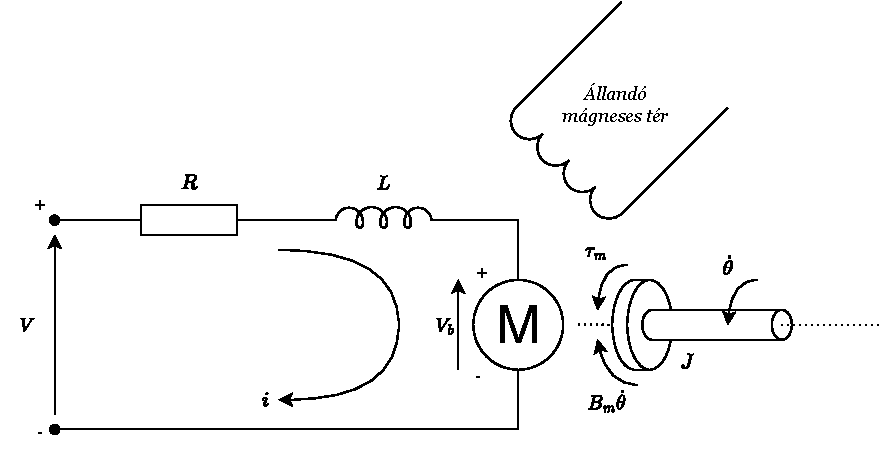
\includegraphics[width=\textwidth]{images/dc_motor_model.pdf}
\caption{Egyenáramú motor áramkör és szabadtest ábra}
\end{center}
\end{figure}

A felhasznált motor feltételezetten állandó gerjesztésű. A kifejtett nyomaték 
a Biot-Savart-törvény szerint arányos a forgorészen átfolyó árammal. A forgórészben
indukált feszültség pedig arányos a szögsebességével a Lenz-törvény alapján 
\begin{align}
    \tau_m = K_\tau i \\
    V_b = K_e \dot\theta
\end{align}
ahol $K_\tau$ a nyomatékállandó, $K_e$ a sebesség-feszültség állandó, $\tau_m$ a kifejtett 
nyomaték, $i$ a rotor árama, $V_b$ az rotorban indukált feszültség és $\dot\theta$ a rotor szögsebessége.
Az energiamegmaradás törvénye alapján a két konstans értéke megegyezik
\begin{align}
    K_m = K_\tau = K_e
\end{align}
így a következőkben $K_m$-ként jelennek meg. A forgorész áramkörére Kirchhoff I. törvénye alapján felírható
\begin{align}\label{eq:armature_circuit}
    V - Ri - L\frac{di}{dt} - K_m\dot\theta = 0
\end{align}
ahol $R$ a forgórész tekercsének ellenállása, $L$ a tekercs induktivitása, 
$K_m$ a motorállandó, $V$ a motor feszültsége, $i$ a motoráram és $\theta$ a szögelfordulás.
A forgórészt mechanikailag egy merev testként tekintve Newton II. törvénye alapján
\begin{align}\label{eq:rotor_dynamics}
    J\ddot\theta = -B_m\dot\theta + K_m i + \tau
\end{align}
ahol $J$ a forgórész tehetetlensége, $B_m$ a viszkózus csillapítási együttható, 
$K_m$ a motorállandó, $\theta$ a szögelfordulás, $i$ a motoráram és $\tau$ a forgórészre
ható külső nyomaték. Ez a két lineáris differenciálegyenlet egyértelműen leírja a 
rendszer időtartománybeli viselkedését.

A további vizsgálathoz kedvezőbb a differenciálegyenleteket állapottérmodellként felírni.
Egy állatopttérmodell általánosan
\begin{align}\label{eq:state_space_generic}
    \dot{\bm x} = \bm A \bm x + \bm B \bm u
\end{align}
\begin{align}\label{eq:state_space_generic_out}
    y = \bm C \bm x + \bm D \bm u
\end{align} 
alakban írható fel. 
A két bemenet a külső nyomaték és a motorra adott feszültség. A kimenet a forgórész szöge.
A paramétereket kifejtve~\ref{eq:armature_circuit} és~\ref{eq:rotor_dynamics} alapján a modell
\begin{align}\label{eq:state_space}
    \frac{d}{dt}
    \begin{bmatrix}
        \theta \\
        \dot\theta \\
        i
    \end{bmatrix}
    =
    \begin{bmatrix}
        0 & 1 & 0 \\
        0 & -\frac{B_m}{J} & \frac{K_m}{J} \\
        0 & -\frac{K_m}{L} & -\frac{R}{L} \\
    \end{bmatrix}
    \begin{bmatrix}
        \theta \\
        \dot\theta \\
        i
    \end{bmatrix}
    +
    \begin{bmatrix}
        0 & 0 \\
        \frac{1}{J} & 0 \\
        0 & \frac{1}{L} \\
    \end{bmatrix}
    \begin{bmatrix}
        \tau \\
        V \\
    \end{bmatrix}
\end{align}
\begin{align}\label{eq:state_space_out}
    \theta = 
    \begin{bmatrix}
        1 & 0 & 0
    \end{bmatrix}
    \begin{bmatrix}
        \theta \\
        \dot\theta \\
        i
    \end{bmatrix}
    +
    \begin{bmatrix}
        0 & 0
    \end{bmatrix}
    \begin{bmatrix}
        \tau \\
        V \\
    \end{bmatrix}
\end{align}
alakba írható át. A frekvenciatartománybeli vizsgálatokhoz felírható a rendszer 
szög-nyomaték és szög-feszültség átviteli függvénye. Az állapottér modellt felhasználva
\begin{align}\label{eq:transfer_generic}
    \frac{Y(s)}{U(s)} = C\left(sI-A\right)^{-1}B+D
\end{align}
általánosan, ahol $I$ az identitás mátrix. Behelyettesítve~\ref{eq:state_space} és~\ref{eq:state_space_out}
paramétereit~\label{eq:transfer_generic} felírható
\begin{align}
    \begin{bmatrix}
        \frac{\theta(s)}{\tau(s)} \\ 
        \frac{\theta(s)}{V(s)} \\ 
    \end{bmatrix}
    =
    \frac{1}{s\left(JLs^2 + \left(B_m L + JR\right)s + K_m^2 + B_m R\right)}
    \begin{bmatrix}
        Ls + R \\ 
        K_m \\ 
    \end{bmatrix}
\end{align}
alakban.

\section{Állapotmegfigyelő}
Az állapotvisszacsatoláshoz szükséges belső állapotok közül csak a szögelfordulás
áll rendelkezésre közvetlen mérésből. A többi állapotra egy megfigyelő ad becslést.
Elkülönítve a mért és becsült állapotokat~\ref{eq:state_space_generic} és ~\ref{eq:state_space_generic_out} felírható
\begin{align}
    \begin{bmatrix}
        \dot\theta \\
        \dot{\bm x}_b
    \end{bmatrix}
    =
    \begin{bmatrix}
        A_{\theta\theta} & \bm A_{\theta b} \\
        \bm A_{b \theta} & \bm A_{bb}
    \end{bmatrix}
    \begin{bmatrix}
        \theta \\
        \bm x_b
    \end{bmatrix}
    +
    \begin{bmatrix}
        B_\theta \\
        \bm B_b
    \end{bmatrix}
    \begin{bmatrix}
        \tau \\
        V \\
    \end{bmatrix}
\end{align}
\begin{align}\label{eq:observer_out}
    \theta = 
    \begin{bmatrix}
        1 & \bm 0
    \end{bmatrix}
    \begin{bmatrix}
        \theta \\
        \bm x_b
    \end{bmatrix}
\end{align}
alakban, ahol $\bm{x}_b$ jelöli a becsült állapotokat. Továbbá jelölje $\tilde{*}$ 
a becsült paramétereket. Ezután legyen
\begin{align}
    \begin{split}
    \hat{\bm A} &= \bm A_{bb} - \bm K_e \bm A_{\theta b} \\
    \hat{\bm B} &= \hat{\bm A} \bm K_e + \bm A_{b \theta} - \bm K_e A_{\theta \theta} \\
    \hat{\bm F} &= \bm B_b - \bm K_e B_\theta
    \end{split}
\end{align}
ahol $\hat{\bm A}$ a megfigyelő belső állapotának (továbbiakban $\tilde{\bm \eta}$) 
dinamikáját adja meg, és $\hat{\bm B}$ és $\hat{\bm F}$ a mért illetve a becsült állapotok 
bemeneti mátrixai. A becsült állapotok és az állapotváltozók közötti összefüggés ekkor
\begin{align}
    \begin{split}
    \bm \eta = \bm x_b - \bm K_e \theta \\
    \tilde{\bm \eta} = \tilde{\bm x}_b - \bm K_e \theta
    \end{split}
\end{align}
alakban adható meg. A belső állapot dinamikája
\begin{align}
    \begin{split}
    \dot{\tilde{\bm \eta}} = \hat{\bm A} \tilde{\bm \eta} + \hat{\bm B} \theta + \hat{\bm F} u
    \end{split}
\end{align}
Végül~\ref{eq:observer_out} átalakításával a rendszer becsült állapotvektora
\begin{align}
    \tilde{\bm x} = \hat{\bm C} \tilde{\bm \eta} + \hat{\bm D} \theta
\end{align}
ahol
\begin{align}
    \hat{\bm C} = 
    \begin{bmatrix}
        \bm 0 \\
        \bm I_{n-1}
    \end{bmatrix},
    \quad
    \hat{\bm D} = 
    \begin{bmatrix}
        1 \\
        \bm K_e
    \end{bmatrix}
\end{align}
mely tartalmazza a mért állapotot is.

\section{Impedancia szabályozó}


\begin{figure}[ht]
\begin{center}
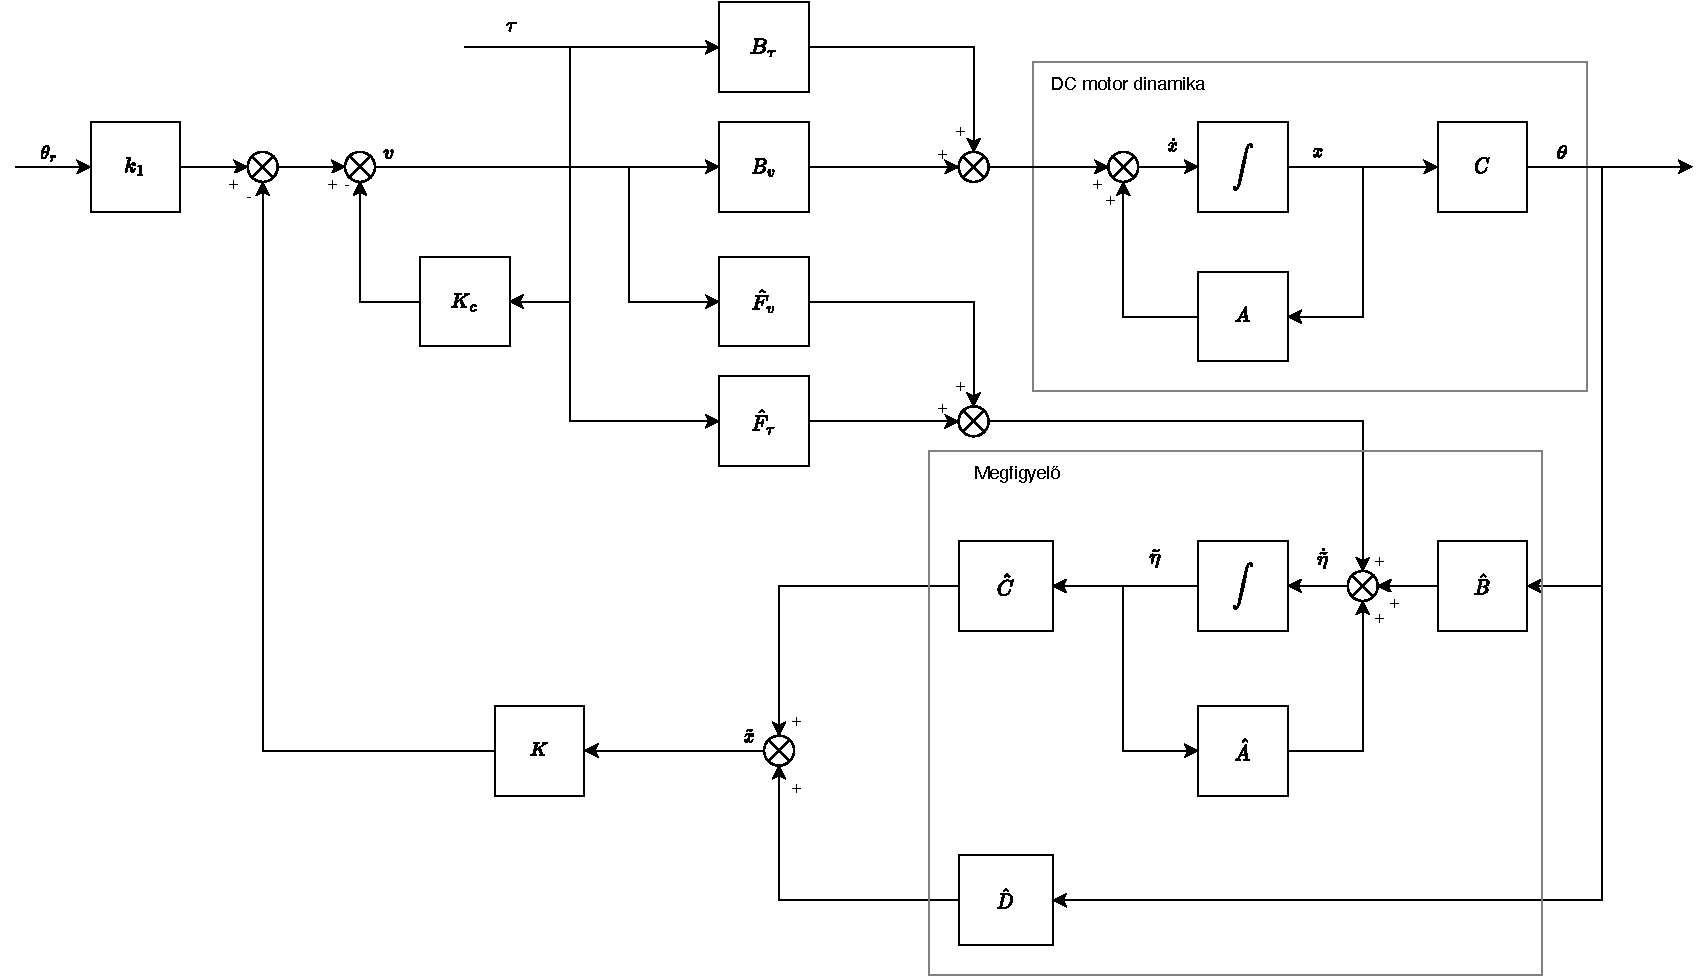
\includegraphics[width=\textwidth]{images/compensated_position_control_torque.drawio.pdf}
\caption{Impedancia szabályozó közvetlen nyomaték méréssel}
\end{center}
\end{figure}

\begin{figure}[ht]
\begin{center}
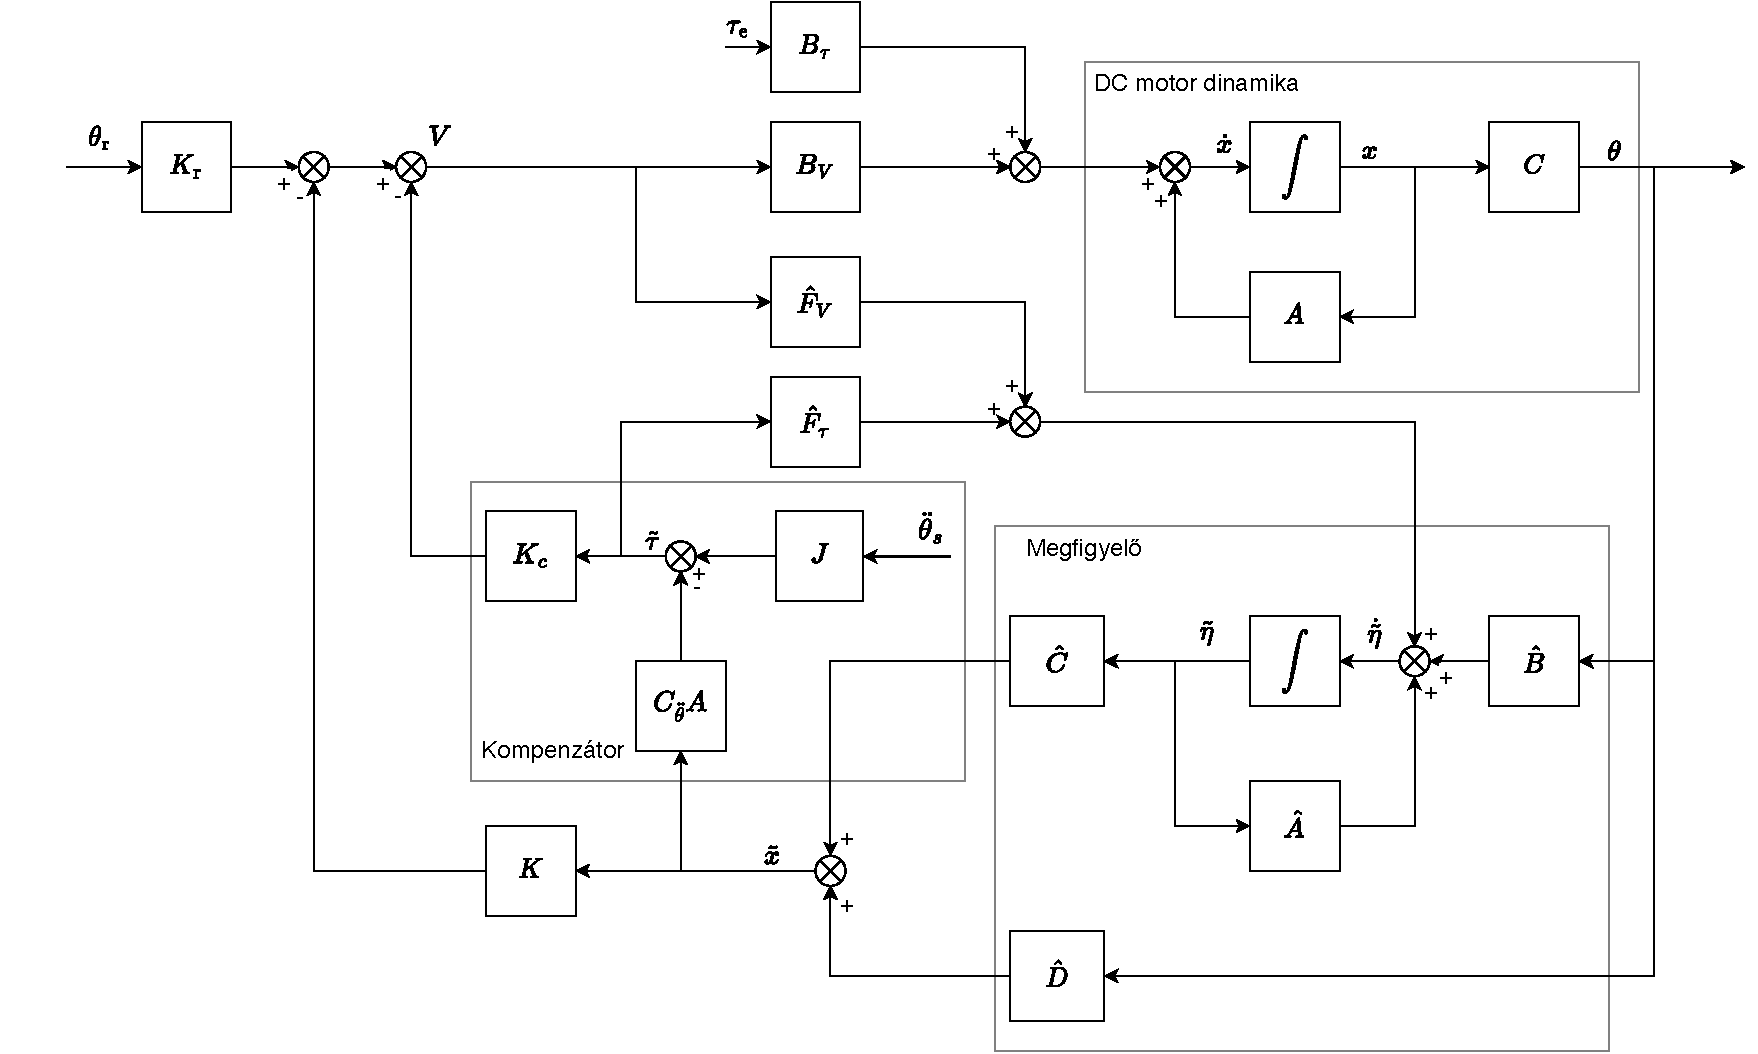
\includegraphics[width=\textwidth]{images/compensated_position_controller_angular_acceleration.pdf}
\caption{Impedancia szabályozó szöggyorsulás méréssel}
\end{center}
\end{figure}


